\documentclass[12pt]{article}
\usepackage{url}
\usepackage[authoryear,round]{natbib}
\usepackage{graphicx} 
\newcommand{\Rpackage}[1]{{\textsf{#1}}}
\newcommand{\Rclass}[1]{{\textit{#1}}}



\title{flowCore: A Bioconductor software package for high throughput flow cytometry analysis}


\author{Florian Hahne*\\
  Nolwenn LeMeur*\\
  Byron Ellis\\
  Ryan R. Brinkman\\
  Perry Haaland\\
  Errol Strain\\
  Deepayan Sarkar\\
  Josef Spidlen\\
  Robert Gentleman
 }

\begin{document}

\maketitle

\section*{Abstract}
\subsubsection*{Background}
Recent advances in automation technologies have enabled the use of
flow-cytometry high content screening (FH-HCS). However, data
management and data analysis methods have not advanced sufficiently
far from the inital small-scale studies to support the large complex
data sets generated in FH-HCS applications.
\subsubsection*{Methods}
In this manuscript, we present \Rpackage{flowCore} a set of flexible
and well structured computational tools for FC-HCS data analysis based
on the open source statistical software R in conjunction with the
Bioconductor Project.
\subsubsection*{Results}
Through \Rpackage{flowCore}, we provide the FCM community a shared
research platform that enables bioinformaticians, computer scientists,
and statisticians to work collaboratively with biologists and
clinicians to develop novel methods for FCM data analysis.
\subsubsection*{Conclusions}
We hope that our framework will be the foundation for fruitful shared
research by many collaborators from multiple scientific fields and
will help resolve bottlenecks that currently prevent the further
development of and deployment of FC-HCS to increasingly complex and
important scientific and clinical applications.

\section*{Introduction}
\subsection*{Computational tools for the analysis of FC-HCS data}
During the last several years, automation technologies have been
developed that enable the use of FCM high content screening
(FC-HCS) to generate large, complex datasets in both basic and
clinical research applications \citep{brinkman2007hcf}. A serious
bottleneck in the interpretation of existing studies and the
application of FC-HCS to even larger, more complex problems is that
data management and data analysis methods have not advanced
sufficiently far from the methods developed for applications of flow
cytometry (FCM) to small-scale, tube-based studies.

Some of the consequences of this lag in development are difficulties
in maintaining the integrity and documentation of extremely large
datasets, assessing measurement quality, developing validated assays,
controlling the accuracy of gating techniques, automating complex
gating strategies, and aggregating statistical results across large
study sets for further analysis.  Among the most serious consequences
of the current situation is, however, that it is very difficult for
new analysis approaches to find there way into standard practice. We
believe that this barrier to the development and dissemination of new
analysis methods is one of the fundamental restraints on the future
expansion of FC-HCS in both clinical and research applications.

In this paper, we describe a set of flexible and well structured
computational tools to efficiently analyze FC-HCS. This set of tools
is based on the open source statistical software R \citep{Rmain}, in
conjunction with the Bioconductor Project \citep{BIOC}. Our intent is
to provide a shared research platform that enables bioinformaticians,
computer scientists, and statisticians to work collaboratively with
biologists and clinicians to develop novel methods for FCM data
analysis, a process deemed crucial by many for the further development
of the technology \citep{lizard2007fca}. A critical component of this
approach is the development and implementation of standards that will
facilitate the adoption of these methods by both the larger research
community and commercial software vendors.  Consequently, we are
optimistic that this software platform will play a critical role in
addressing the bottlenecks described above that limit further advances
in the application of FC-HCS.

The computational tools we have developed are distributed in the R
software language as the Bioconductor package
\Rpackage{flowCore}. \Rpackage{flowCore} is a freely available, highly
functional and extensible FCM data analysis platform that enables
researchers to efficiently handle FC-HCS data and encourages open
development of tools for their coherent analysis. Among the issues
addressed by \Rpackage{flowCore} are computationally efficient data
structures and a range of specialized methods for compensation,
transformation, and gating.  \Rpackage{flowCore} runs on Windows, Mac
OS X and Linux/Unix operating systems. Conceptually, the underlying
data structures that build the core of our software can be implemented
in any programming language, and we chose the R language for its
advantages in statistical programming and visualization. In this
paper, we describe the functionality and methods underlying
\Rpackage{flowCore}, and provide examples of their use.

\subsection*{R and Bioconductor}
R is a robust statistical programing environment which offers a wide
range of statistical and visualization methods developed for various
fields of application. In particular, the Bioconductor project
provides R software modules for biological and clinical data analysis.
It is widely used to process such data, spanning a diversity of
research fields including genomics, proteomics and cell biology
\citep{BIOC}. The R language and Bioconductor are
particularly geared towards the analysis of large complex datasets
that typically arise from high throughput experiments such as
microarray gene expression analysis or FC-HCS. Using FCM as
a high-throughput technology requires suitable software infrastructure
to facilitate the rapid handling of the data. In our implementation of
\Rpackage{flowCore} we rely on two important lessons learned from the field of
gene expression data analysis: the first being the importance of data
structures that reflect the underlying data and facilitate the
manipulations that are of most interest, while the second is the
importance of a modular architecture that allows for many developers
to extend and use the underlying infrastructure and to combine tools
in complex work flows.

\subsection*{Existing data standards and conventions}
Traditionally, the majority of FCM experiments have been analyzed by
manual data inspection in one or two dimensions, or by very basic
comparisons of summary statistics and most of the currently available
analysis tools are designed to reflect this workflow.  We believe that
these approaches, in addition to being expensive and labor intensive,
do not fully address the highly complex nature of FCM data; in
particular, they disregard many of the fundamental aspects of the
data, such as its underlying distribution and its high-dimensional
nature. Furthermore, the subjective character of manual analyses are a
major obstacle to reproducibility. For FC-HCS data, unassisted manual
inspection is extremely time consuming, and robust statistical methods
need to be developed to point investigators to interesting aspects of
the data, or to potential problems. While the expert knowledge of
immunologists and researchers remains crucial for the understanding of
FCM data, we believe that collaboration with other research fields
such as statistics and computer science can greatly improve the
relevance of FCM in today's high-throughput paradigm.

Currently, data from FCM experiments are stored in single files
according to the Flow Cytometry Standard (FCS) \citep{seamer1997pnd}.
However, recent developments in high-throughput FCM are shifting the
focus of interest away from single-tube based measurements towards
large and complex experimental designs with dozens of covariates and
influencing factors. For example, experiments consist of large numbers
of samples from different patients, measured at different timepoints
\citep{brinkman2007hcf} or following different drug treatments
\citep{gasparetto2004ice}. Modern FCM data analysis tools have to deal
with an additional layer of sample metadata and they need to provide
infrastructure to process and to compare groups of samples in a
concise and coordinated manner.

The notion of classes from an object-oriented programming language
provides one coherent way to describe these richer data structures,
and functions or methods that work on them allow for interaction and
manipulation. Many of the currently available software solutions offer
only limited support for such self-contained structures, or make use
of containers like XML or binary storage formats that are designed
specifically for particular user interfaces and hence are not easily
amenable to programmatical access. In addition, the closed-source
nature of these products often makes it impractical to integrate them
into analysis pipelines. In this manuscript we describe classes for
FCM data analysis and their implementation in R, however, they could
just as easily be implemented in any other language (e.g., Java,
C++). Software written in those languages could use similar data
structures, thereby simplifying communication and the interchange of
data between analysis tools.

The \Rpackage{flowCore} framework presented here can import and
process raw data FCS files along with their complete set of
file-specific metadata (Figure~\ref{fig1:FrameWork}).  Moreover, it is
a software implementation of the Gating-ML CR, an new flow
cytometry data standard developed in collaboration with the ISAC Data
Standards Task Force, which makes it possibile to integrate
\Rpackage{flowCore} in existing work flows and to communicate with any
other FCM tool that adheres to the proposed standard\citep{SpidlenInPressCytometryA}. Adherence to
standards also plays a critical role in the ability of new methods
based on \Rpackage{flowCore} to find their way back into the standard
practices for FCM data analysis. \Rpackage{flowCore} is not a
GUI-driven software, and all operations are done using a command line
interface.  It is possible to add a more elaborate user interface on
top of this infrastructure, however the focus in this paper is on a
programmatic approach to enable the convenient development of novel
analysis methods and automation of complex analysis approaches.  By
taking the burden of data management from the programmer, and by
providing well-defined programming interfaces (APIs), it is possible
to readily test new ideas and to easily extend the framework's
functionality.



\section*{Materials and Methods}
\subsection*{Basic data structures}
\subsubsection*{flowFrame}

\Rpackage{flowCore}'s primary task is the representation and basic
manipulation of FCM data. This is accomplished through a data model
very close to that adopted by other Bioconductor packages. All
information from a single FCS file, i.e., the collection of events and
the accompanying metadata, is stored in one single container. We call
the structure that hold this data a \Rclass{flowFrame}. Raw data
values as well as associated metadata of a \Rclass{flowFrame} can be
accessed programmatically. Most commonly, the metadata consist of
descriptors of the stains used in the experiment and the respective
measurement channels, information about compensation performed at the
instrument side and any additional keywords the user deems to be
important to annotate the data. A number of quality checks are
performed during the creation of a \Rclass{flowFrame} to ensure data
integrity.

\subsubsection*{flowSet}
In high-throughput FCM, many of the analysis tasks need to be
performed consistently across multiple flow measurements, hence we
introduce the concept of a collection of \Rclass{flowFrames} called a
\Rclass{flowSet}. A \Rclass{flowSet} is a container for multiple
\Rclass{flowFrames} along with relevant information associated with
each individual frame such as descriptions of the cell sample, the
treatment to which the sample was subjected, or the location of that
sample in a 96 or 384 well plate.  \Rclass{flowSets} manage the
consistent application of operations on the individual
\Rclass{flowFrames} and shift the burden of keeping score of the
metadata from the user to the infrastructure, thus reducing the risk
of errors (\textit{e.g.}, mixups of sample labels). The
\Rclass{flowSet} structure can be readily extended to incorporate the
potentially complex metadata associated with even larger FC-HCS
experiments such as clinical trials where hundreds patients might
provide samples at different points in time over the course of the
experiment.


%%Figure1 Diagram of the data structures and the basic operations
\begin{figure}
\centering
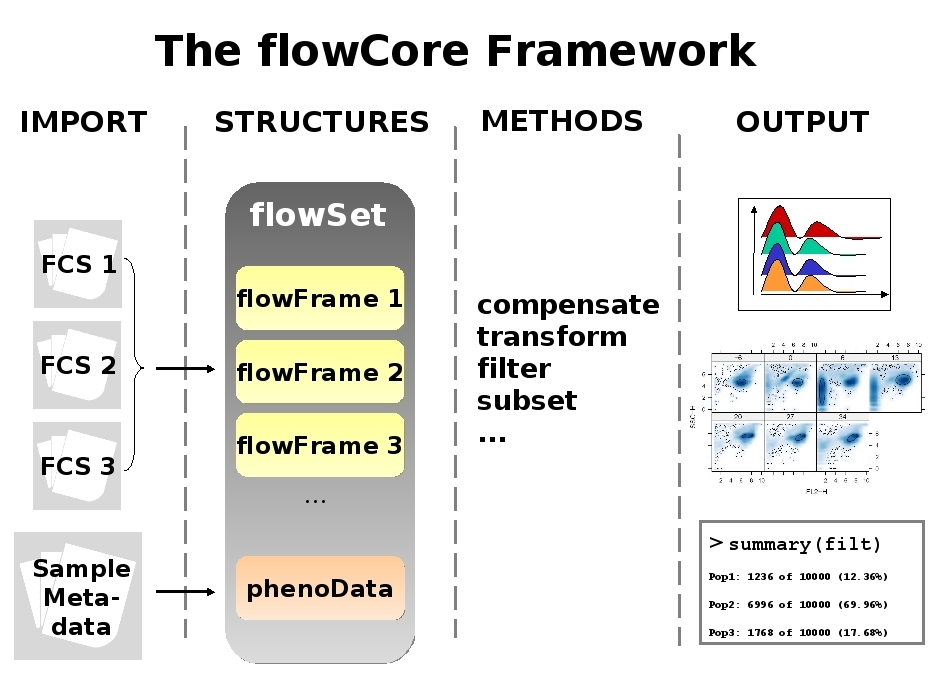
\includegraphics[width=0.9\textwidth]{Figure1-flowCoreFrameWork.jpg}
\caption{\label{fig1:FrameWork}{For each experiment, FCS files (as
    individual \Rclass{flowFrames}), phenotypic and metadata are
    stored in a \Rclass{flowSet}. Each \Rclass{flowFrame} in a
    \Rclass{flowSet} corresponds to one FCS file. All basic operations
    (e.g., compensation, transformation, gating) can be applied to
    either single \Rclass{flowFrames} or a \Rclass{flowSet}
    simultaneously.}}
\end{figure}




\subsection*{Standard flow operations}

The basic operations in FCM analyses are typically the same: the data
need to be compensated (if that was not already done on the
instrument) and transformed, and sup-populations of interest need to
be selected based on a set of (predominantly sequential) gates. All
software solutions for FCM analysis offer support for these
operations, typically in an interactive, GUI-driven interface. The
approach we have taken in \Rpackage{flowCore} is to abstractly
describe these operations and build a set of tools to perform them on
both \Rclass{flowFrames} and \Rclass{flowSets}. While transformation,
and to a certain extent compensation, are fairly routine operations
with only limited potential for improvement, being able to implement
new methodologies for gating of FCM data, and extending the
capabilities of \Rpackage{flowCore} through object oriented
programming are features that clearly sets our framework apart from
other FCM analysis tools. By factoring out as much of the bookkeeping
as possible, programmers can focus on the actual operations rather
then having to deal with the tedious details of data integration and
access. Third-party methods can act on their own as first-class
citizens in the analysis framework, without breaking the work flow or
the basic infrastructure. This design allows for the straightforward
extension of \Rpackage{flowCore}'s capabilities, and has already
fostered the development of a number of valuable add-ons
\citep{lo2008agf,sarkar2008ufv} \textit{(Fixme Errol: Will plateCore
  be in Bioconductor soon. It should be if we want to cite it.)}.

\subsubsection*{Transformation and compensation}

Data transformation is essential for both data visualization and
modelling \citep{lo2008agf}. The major transformations that are
routinely used in FCM analysis have been implemented in
\Rpackage{flowCore} (\textit{e.g.,} quadratic, log or arcsinh, see
Table~\ref{table1} for a complete list). Furthermore, the design of
the R language makes it easy to define arbitrary functions to apply to
the data of individual \Rclass{flowFrames} or entire
\Rclass{flowSets}, respectively. Compensation is available for both
\Rclass{flowFrames} and \Rclass{flowSets}, and the software also
offers functionality to compute spillover or compensation matrices
from a set of appropriate compensation samples.

\begin{table}[ht]
\begin{center}
\begin{tabular}{|l|l|}
\hline
\multicolumn{2}{|c|}{Data Transformations} \\
\hline
linear & $ax + b$ \\
quadratic & $ax^2 + bx + c$ \\
natural logarithm & $ln(x)(r/d)$ \\
logarithm & $log(x)(r/d)$ \\
biexponential & $root(a*e^{(b*y)}-c*e^{(-d+y)}+f)$ \\
logicle& $root(Te^{-(m-w)}*(e^{(y-w)}-p^2e^{-(y-w)/p}+p^2-1)$ \\
truncate & $x_{x<=a} = a$ \\
scale & $(x-a)/(b-a)$ \\
split-scale & combination of linear and logarithm \\
arcsinh & $asinh(a + bx)+c$ \\
\hline
\end{tabular}
\caption{\label{table1}Data transformations implemented in
  \Rpackage{flowCore}.}
\end{center}
\end{table}

\subsubsection*{Gating}
%%FIXME: I would make more of the filters and possibly try to make it
%%clearer how much stuff thre is for composition of gates/filters etc
%%
%% somewhere notions of apply and summary methods should appear and if
%% we have anything figured out yet on how to do the subsetting etc
%% that too would go nicely in here (here I am thinking of our
%% discussion of the sort of workflow stuff)

In \Rpackage{flowCore}, gating operations are represented by classes
that can be extended in an object-oriented manner
(Table~\ref{table2}). Basic gate types such as rectangular gates,
ellipses and polygon gates are implemented as part of the
framework. In addition, we introduce the notion of data-driven gates,
or filters, for which the necessary parameters are computed based on
the properties of the underlying data, for instance by modelling data
distribution or by density estimation. This approach is fundamentally
different from the traditional application of static gating regions
across samples, as it is able to take into accounts unforeseen changes
in signal intensities (\textit{e.g.,} drifts in the instrumentation
over time or sample variablity).

The ability to programmatically access gates is a prerequisite for
automated or semi-automated gating. By utilizing a unified interface
for all different types of gates, the user is able to subset data sets
as well as to create summary statistics, for example the proportions
of events falling in a single gate or in a combination of
gates. Complex combinations and hierarchies of gates can be captured
in objects of class \Rclass{filterSet}, allowing to apply multi-step
gating strategies. The definition of gates in \Rpackage{flowCore}
follows the Gating-ML CR, thus any \Rpackage{flowCore} gating strategy
can be reproduced by any other software that also adheres to the
standard.

Gating, as well as all other operations in flowCore, can be applied
over each individual frame in a \Rclass{flowSet}, and summary methods
provide information about the outcome of these operations. In
addition, the result of a gating operation can be used to subset the
input \Rclass{flowFrame} or \Rclass{flowSet}, either by filtering out
negative events or by splitting in multiple subpopulations. This
design allows to easily combine all of \Rpackage{flowCore}'s
components into complex work flows.

\begin{table}[ht]
\begin{center}
\begin{tabular}{|l|l|}
\hline
\multicolumn{2}{|c|}{Gates} \\
\hline
rectangleGate & n-dimensional rectangular regions \\
quadGate & quadrant regions in two dimensions \\
polygonGate & polygonal regions in two dimensions \\
polytopeGate & generalization of polygon in n dimensions \\
ellipsoidGate & n-dimensional ellipsoid region \\
\hline
\multicolumn{2}{|c|}{Filters} \\
\hline
sampleFilter & random sub-sampling\\
expressionFilter & results of a boolean expression \\
kmeansFilter & K-means clustering \\
norm2Filter & bivariate normal distribution \\
curv1Filter & local density regions in 1D \\
curv2Filter & density regions in 2D \\
timeFilter & abnormal data acquisition over time \\
\hline
filterSet & gating strategies \\
\hline
\end{tabular}
\caption{\label{table2}Filter and gate classes implemented in
  \Rpackage{flowCore}.}
\end{center}
\end{table}

\subsection*{Related flow packages}

In addition to the \Rpackage{flowCore} package that offers basic
infrastructure, we have implemented a range of additional Bioconductor
packages that are dedicated to more specific tasks of FCM data
analysis. The \Rpackage{flowViz} package \citep{sarkar2008ufv}
provides sophisticated data visualization tools, that make use off
multivariate trellis plotting \citep{lattice}.  These functions can be
used to quickly generate customized plots for extended cytometry data
sets for both direct data inspection and quality control.  The objects
metadata information can be used to arrange the layout and composition
of the plots.  Furthermore, the design and the API of the
visualization software is very generic, and users can readily extend
its capabilities by providing self-defined plotting functions.  The
\Rpackage{flowQ} package offers more advanced quality assurance (QA)
methodology and a framework to create interactive web-based reports of
QA results.  Most of \Rpackage{flowUtil}'s content deals with data
import and export, implementing the flow-cytometry specific standard
markup language.  Finally, \Rpackage{flowStats} provides more
elaborate statistical methods that are relevant in the context of flow
cytometry data analysis. \cite{lo2008agf} have recently developed an
automatic gating approach via robust model-based clustering using
\Rpackage{flowCore}'s data model and infrastructure which is
implemented in the Bioconductor package \Rpackage{flowClust}. Another
package, \Rpackage{plateCore}, providing more specialized support for
experiments conducted on microtitre plates and facilitiating the
handling of spatial metadata, is under development.

\section*{Results}
The \Rpackage{flowCore} package has been successfully applied in the
analysis of several datasets
\citep{gasparetto2004ice,brinkman2007hcf}. A complete documentation of
the \Rpackage{flowCore} software is beyond the scope of this
publication.  Much more comprehensive documentation and users guide
information with programmatic examples is available online
(\url{http://bioconductor.org/packages/2.2/bioc/html/flowCore.html})
and as part of the package distribution. Here, we want to briefly
exemplify some of the software's key features, that is, the coherent
treatment of all samples in a potentially large experiment, the
concept of data-driven automated gating, the integration of existing
software into the framework, and the generation of publication-quality
graphics for data visualization.

Data analysis for most experiments usually begins with a quality
assurance step, and we can use functionality from the \Rpackage{flowQ}
package to create an HTML report that highlights potential quality
issues. Assuming that the data has already been imported as the
\Rclass{flowSet} object ``dat'', the following simple line of code
produces the output shown in Figure~\ref{flowQ}:

\begin{verbatim}
> library(flowCore)
> library(flowQ)
> qaReport(dat, c("qaProcess.timeline", "qaProcess.timeflow", 
                  "qaProcess.cellnumber"))
\end{verbatim}

The report is interactive and provides drill-down to more detailed
aspects of the analysis, starting from a concise overview. The design of \Rpackage{flowCore}'s data model
allows for a coherent treatment of all the samples, hence we are able
to compare features between individuals, or between groups of
individuals, based on the available metadata information.


\begin{figure}[htbp]
\centering
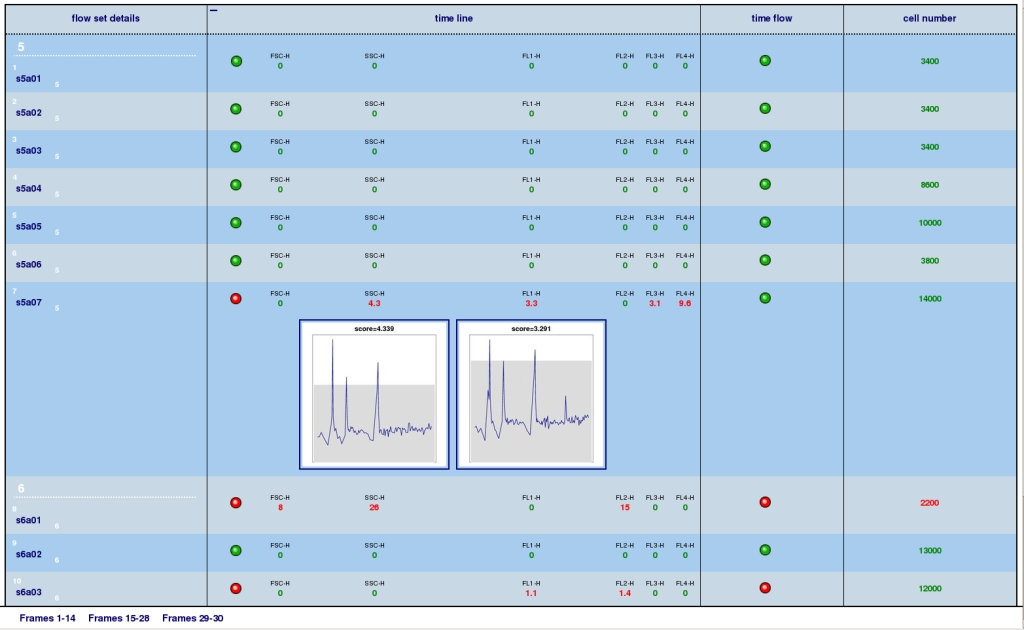
\includegraphics[width=0.75\textwidth]{flowQ.jpg}
\caption{\label{flowQ}%
  HTML quality assessment report generated by the flowQ package. Rows
  correspond to samples, columns to different quality checks.}
\end{figure}

Static gating for all samples in a high-throughput FCM experiment is
often not an option, since the measured variables tend to vary between
different treatments, over time or between different experiment
batches. Automated or data-driven gating tries to estimate the gating
regions from the underlying data, thus providing a fast objective
solution to the analysis of potentially very large and diverse data
sets \cite{lo2008agf}. One of the automated gating methods implemented
in \Rpackage{flowCore} is based on identifying areas of significant
curvature in a kernel density estimate of the data
\citep{wand2008}. Assuming that the regions of interest are of high
density, the software is able to reliably detect them in a one or
two-dimensional density landscape.

\begin{verbatim}
> cf <- curv2Filter("FL1-H", "FL3-H")
> fres <- filter(dat, cf)
\end{verbatim}

Kernel density estimation is a well-known problem in statistical
computing, and a lot of effort has been invested in the development of
good software to address it. The modular design of \Rpackage{flowCore}
allows to easily integrate these existing solutions into our
framework. In this example, we directly use R code from the
\Rpackage{feature} package developed by \cite{wand2008}. Instead of
re-writing existing code, we are able to include it via the well
tested distribution mechanism provided by R's software package
system. This process is bi-directional, and all functionality
implemented in \Rpackage{flowCore} is available to other package
authors, as we have seen with the afore-mentioned \Rpackage{flowClust}
package.

We can chose one of the many visualization option from the flowViz
package to plot the results of the recent filtering operation. A very
basic matrix of density plots is shown in Figure \ref{xyplot}, where
each panel in the matrix represents the data of one individual
patient.

\begin{verbatim}
> xyplot(`FL1-H` ~ `FL3-H` | SampleID, data=dat, filter=fres)
\end{verbatim}


\begin{figure}[htbp]
\centering
\includegraphics[width=0.75\textwidth]{xyplot}
\caption{\label{xyplot}%
  Scatterplot matrix of a single \Rclass{flowSet} with outlines of the
  gating regions identified by an automated gating operation.}
\end{figure}



\section*{Discussion}

Through \Rpackage{flowCore}, we have provided the FCM community an open source,
freely available, highly functional, standards compliant development
and analysis platform for high throughput data analysis.  Our
intention is to provide a platform for the collaborative development
of new analysis methods that will facilitate the transition of these
new methods to the larger flow community.  Our experience has been
that the collaborative effort we enable for devising new methodology
has been proven beneficial for a number of different biological and
computational biology challenges.  We hope that our framework will be
the foundation for fruitful shared research by many collaborators from
multiple scientific fields and will help resolve bottlenecks that
currently prevent the further development of and deployment of FC-HCS
to increasingly complex and important scientific and clinical
applications.

\section*{Acknowledgements}
This work was supported by NIH grant EB005034 and by the Michael Smith
Foundation for Health Research. RRB is an ISAC Scholar.

\bibliographystyle{plainnat}  
\bibliography{flowCoreRef} 
\end{document}

